\documentclass{article}
\usepackage{amsmath}
\usepackage{graphicx}
\usepackage{listings}
\usepackage{hyperref}
\usepackage{color}
\usepackage[backend=biber,style=numeric,citestyle=numeric]{biblatex}
\addbibresource{references.bib}

\title{Airbnb Price Prediction Using CRISP-DM Methodology}
\author{Jayanth Kalyanam \\ San Jose State University \\ \texttt{jayanth.kalyanam@sjsu.edu}}
\date{\today}

\begin{document}

\maketitle

\begin{abstract}
This paper presents a comprehensive data science project focused on predicting Airbnb rental prices in New York City using the CRISP-DM methodology. By leveraging machine learning techniques such as XGBoost, the paper explains each phase of the project in detail, from data understanding and preparation to modeling and deployment. The final model is deployed using a Flask API, allowing real-time price prediction for Airbnb listings.
\end{abstract}

\section{Introduction}
The Airbnb market in New York City is highly competitive, and accurate pricing plays a crucial role in maximizing occupancy rates. This paper aims to predict rental prices based on multiple features, using the CRISP-DM framework. This process includes data understanding, preparation, modeling, and evaluation, culminating in deploying the final model as a Flask API. Machine learning models, including Linear Regression, Random Forest, Gradient Boosting, and XGBoost, are compared to determine the best model for predicting Airbnb rental prices.

\section{CRISP-DM Methodology}

\subsection{Business Understanding}
The business goal is to predict Airbnb rental prices to help hosts optimize their listings and maximize earnings. Accurately predicting rental prices can improve competitiveness, helping hosts set prices that balance revenue and occupancy rates. Key questions include:
\begin{itemize}
    \item Which factors influence rental prices the most?
    \item How accurately can machine learning models predict Airbnb rental prices?
\end{itemize}

\subsection{Data Understanding}
The dataset used in this project is the Airbnb NYC 2019 dataset from Kaggle, containing over 48,000 listings. The features include numerical attributes like `price`, `minimum\_nights`, and `availability\_365`, and categorical attributes like `neighbourhood\_group` and `room\_type`.

Here, we perform exploratory data analysis (EDA) to understand the data and visualize key distributions and correlations.

\begin{figure}[h!]
    \centering
    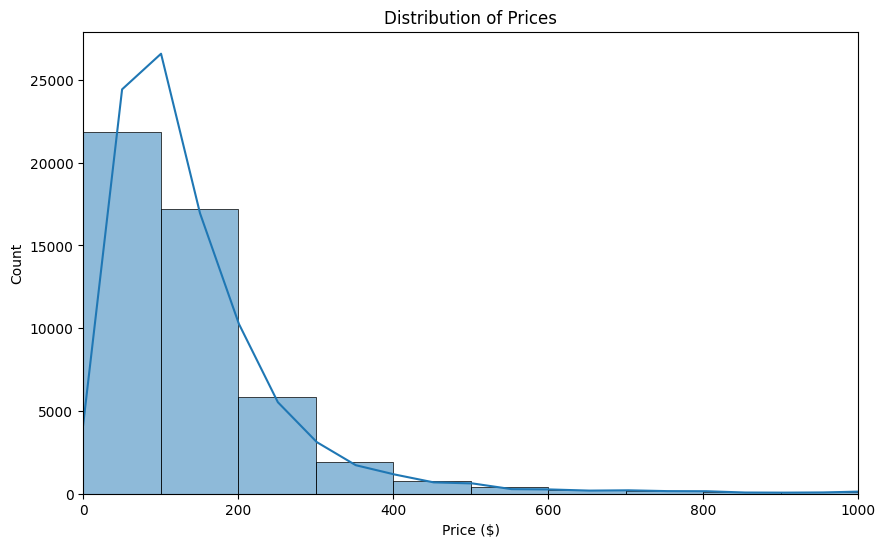
\includegraphics[width=0.7\textwidth]{price_distribution.png}
    \caption{Price Distribution for Airbnb Listings}
\end{figure}

\subsection{Data Preparation}
The following steps were undertaken to preprocess the data:
\begin{itemize}
    \item Handling missing values in `reviews\_per\_month` by filling them with 0.
    \item Removing outliers by capping prices at the 99th percentile.
    \item Log-transforming the target variable `price` to normalize its distribution.
    \item Encoding categorical features like `neighbourhood\_group` and `room\_type` using one-hot encoding.
    \item Standardizing numerical features such as `latitude`, `longitude`, `availability\_365` using `StandardScaler`.
\end{itemize}

\begin{lstlisting}[language=Python]
# Fill missing values
df['reviews_per_month'].fillna(0, inplace=True)

# Cap prices at the 99th percentile
price_cap = df['price'].quantile(0.99)
df = df[df['price'] <= price_cap]

# Log-transform the price
df['log_price'] = np.log1p(df['price'])

# One-hot encoding for categorical variables
df = pd.get_dummies(df, columns=['neighbourhood_group', 'room_type'], drop_first=True)

# Standardizing numerical features
scaler = StandardScaler()
numerical_features = ['latitude', 'longitude', 'minimum_nights', 'availability_365']
df[numerical_features] = scaler.fit_transform(df[numerical_features])
\end{lstlisting}

\subsection{Modeling}
Four machine learning models were trained to predict the log-transformed price: Linear Regression, Random Forest, Gradient Boosting, and XGBoost. After splitting the data into training (80\%) and test (20\%) sets, we evaluated each model using performance metrics such as Mean Absolute Error (MAE), Root Mean Squared Error (RMSE), and R-squared (R²).

\begin{lstlisting}[language=Python]
from sklearn.model_selection import train_test_split
import xgboost as xgb

# Split data into training and test sets
X = df.drop(['log_price'], axis=1)
y = df['log_price']
X_train, X_test, y_train, y_test = train_test_split(X, y, test_size=0.2, random_state=42)

# Train XGBoost model
xgb_model = xgb.XGBRegressor(random_state=42, objective='reg:squarederror')
xgb_model.fit(X_train, y_train)
\end{lstlisting}

\section{Evaluation}
The XGBoost model performed the best among all models, achieving an MAE of 0.29, RMSE of 0.40, and an R² of 0.64. The table below compares the performance metrics for all the models:

\begin{tabular}{lccc}
\hline
Model & MAE & RMSE & R² \\
\hline
Linear Regression & 0.33 & 0.44 & 0.57 \\
Random Forest & 0.30 & 0.41 & 0.63 \\
Gradient Boosting & 0.31 & 0.42 & 0.61 \\
XGBoost & 0.29 & 0.40 & 0.64 \\
\hline
\end{tabular}

We used XGBoost's feature importance to identify the key factors influencing price predictions. The most significant features included `private room`, `shared room` and `neighbourhood`.

\begin{figure}[h!]
    \centering
    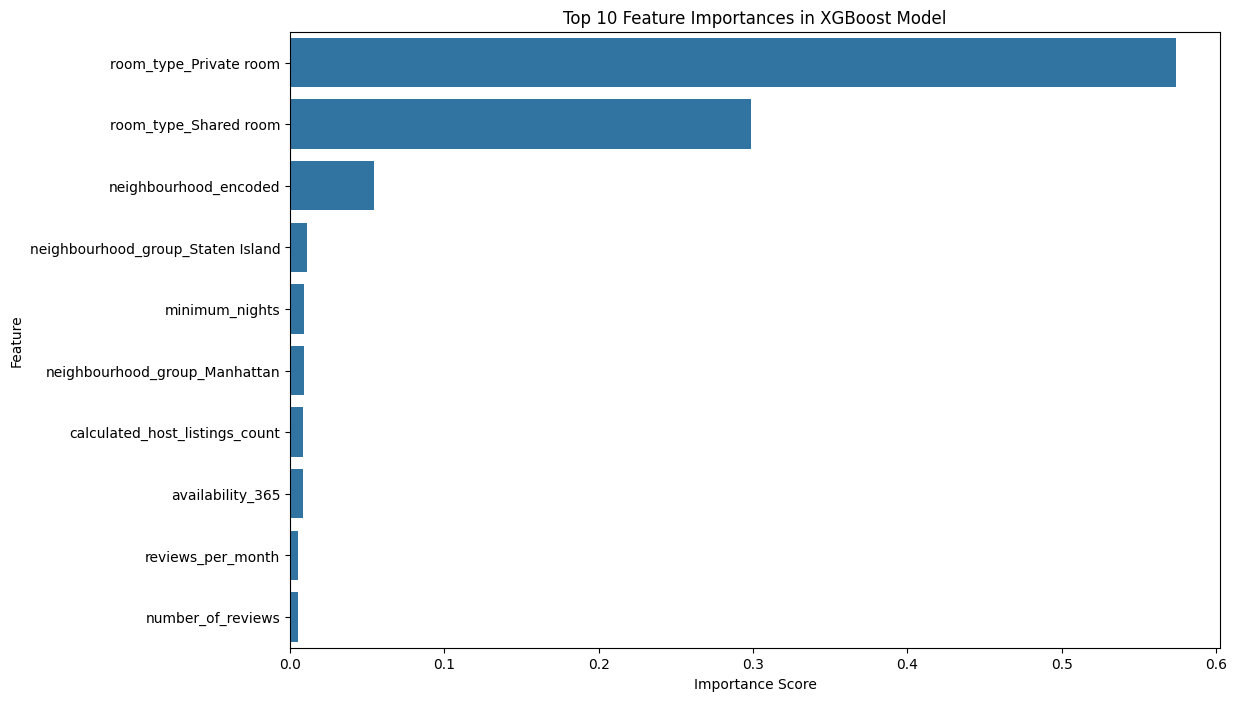
\includegraphics[width=0.7\textwidth]{feature_importance.png}
    \caption{Feature Importance in XGBoost Model}
\end{figure}

\section{Deployment}
The trained XGBoost model was deployed using a Flask API. The API accepts a JSON payload containing the feature values and returns the predicted price. This allows hosts to obtain real-time price predictions for their listings.

\begin{lstlisting}[language=Python]
from flask import Flask, request, jsonify
import joblib
import pandas as pd
import numpy as np

# Load model and scaler
model = joblib.load('xgb_model.pkl')
scaler = joblib.load('scaler.pkl')

app = Flask(__name__)

@app.route('/predict', methods=['POST'])
def predict():
    try:
        data = request.get_json(force=True)
        input_df = pd.DataFrame([data])
        input_df = preprocess_input(input_df)
        prediction_log_price = model.predict(input_df)
        prediction_price = np.expm1(prediction_log_price)
        return jsonify({'predicted_price': float(prediction_price[0])})
    except Exception as e:
        return jsonify({'error': str(e)})
\end{lstlisting}

\section{Conclusion}
By following the CRISP-DM methodology, this project built and deployed a machine learning model that successfully predicts Airbnb rental prices. XGBoost performed the best in terms of accuracy. The model was deployed via a Flask API, enabling real-time price predictions for Airbnb hosts. This project demonstrates the importance of structured data preparation, careful model selection, and efficient deployment strategies in real-world machine learning applications.

\section{References}
\nocite{*}
\printbibliography


\end{document}
